\documentclass[10pt, english]{report}

\usepackage{hyperref}

\usepackage{float}


%encoding
%--------------------------------------
\usepackage[utf8]{inputenc}
\usepackage[T1]{fontenc}
%--------------------------------------

%French-specific commands
%--------------------------------------
\usepackage{babel}
\usepackage[autolanguage]{numprint}
%--------------------------------------

%Hyphenation rules
%--------------------------------------
\usepackage{hyphenat}
\hyphenation{mathéma-tiques récu-pérer}
%--------------------------------------

%Maths box
%--------------------------------------
\usepackage{amsmath}
\usepackage[most]{tcolorbox}

\tcbset{colback=yellow!10!white, colframe=red!50!black, 
	highlight math style= {enhanced, %<-- needed for the ’remember’ options
		colframe=red,colback=red!10!white,boxsep=0pt}
}
%--------------------------------------

%code blocs
%--------------------------------------

\usepackage{listings}
\usepackage{xcolor}

\definecolor{codegreen}{rgb}{0,0.6,0}
\definecolor{codegray}{rgb}{0.5,0.5,0.5}
\definecolor{codepurple}{rgb}{0.58,0,0.82}
\definecolor{backcolour}{rgb}{0.95,0.95,0.92}

\lstdefinestyle{mystyle}{
	backgroundcolor=\color{backcolour},   
	commentstyle=\color{codegreen},
	keywordstyle=\color{magenta},
	numberstyle=\tiny\color{codegray},
	stringstyle=\color{codepurple},
	basicstyle=\ttfamily\footnotesize,
	breakatwhitespace=false,         
	breaklines=true,                 
	captionpos=b,                    
	keepspaces=true,                 
	numbers=left,                    
	numbersep=5pt,                  
	showspaces=false,                
	showstringspaces=false,
	showtabs=false,                  
	tabsize=2
}

\lstset{style=mystyle}
%--------------------------------------

\usepackage[margin=2cm]{geometry}
\usepackage{graphicx}

\title{
	
\includegraphics[scale=1]{img/logo.png}\\[4cm]
	\huge\textbf{Natural Language Processing for Fact-Checking and Claim Assessment}\\[1cm]
	\Large{Intermediate report of project advancement} \\[4cm]
}
\author{
	Othman EL HOUFI\\
	Dimitris KOTZINOS \\[0.5cm]
	\textbf{MSc Research in Data Science \& Machine Learning} \\[1.5cm]
}

\date{\today}

\begin{document}
	
	%%%%%TITLE%%%%%
	\begin{titlepage}
		\maketitle
	\end{titlepage}

\chapter*{Abstract}
As false information and fake news are propagating though out the internet and social networks, the need of fact-checking operations becomes necessary in order to maintain a truthful digital environment where general information can be reliably exploited whether in politics, finance and other domains. The need of this online claim assessment comes from the fact that fake news and false information can have a big negative impact on politics, economy (2016 USA Elections) and public health (COVID-19).\\ 
A number of solutions have been proposed to deal with this problem and limit the spread of false information, both manual and automatic. Of course the manual approaches done on websites such as \textit{PolitiFact.com}, \textit{FactCheck.org} and \textit{Snopes.com} don't construct a viable solution for the long term as the speed and scale of information propagation increase exponentially rendering this manual fact-checking operation where human fact-checkers can't scale up at the same rate limited and incapable of solving the problem.\\
Here, we present our contribution in this regard: an automated solution for fact-checking using Wikipedia's articles for claim verification. The algorithm uses NLP techniques in order to extract the so-called claim from the user input, then, using Wikipedia's API, it retrieves all the relevant articles and assesses with a degree of confidence if the claim is true, false or unable to decide due to lack of information showing evidence (sentences in articles) and probabilities for each resulted case.\\[1cm]

\textbf{Keywords:} Natural Language Processing, Wikipedia, Information retrieval, Text processing, Natural Language Inferencing, Fact-Checking, Document retrieval, Sentence retrieval, Fake-news.

%%%%%TABLE OF CONTENT%%%%%
\tableofcontents

\chapter{Introduction}
\section{Project Context}

From a social and psychological perspective, humans have been proven irrational and vulnerable when differentiating between truth and false news (typical accuracy ranges between 55\% and 58\%), thus fake news obtain public trust relatively easier than truthful news because individuals tend to trust fake news after repeated exposure (\textit{Validity effect}), or if it confirms their pre-existing beliefs (\textit{Confirmation bias}), or simply due to the obligation of participating socially and proving a social identity (\textit{Peer pressure}). The social sciences are still trying to comprehend the biological motivations that makes fake news more appealing to humans.\\

On the other hand, the growth of social media platforms resulted in a huge acceleration of news spreading whether true or false. As of Aug. 2017, 67\% of Americans get their news from social media. These platforms even give the user the right to share, forward, vote and participate to online discussions. All of this made the problem of fake news spreading more and more dangerous, our economies for example, are not robust to the spread of falsity, false rumors have affected stock prices and the motivations for large-scale investments, as we witnessed after a false tweet claimed that Barack Obama was injured in an explosion which caused \$130 billion drop in stock value. Another recent example is related to public health where rumors about COVID-19 vaccines and drug companies influenced people in their decision on getting vaccinated.\\

That being said, is there a way to monitor the spread of fake news through social media? Or more specifically, how can we differentiate between fake news and truthful news, and at what level of confidence can we do that?\\

From a computer engineering perspective, different approaches were studied:

\begin{itemize}
\item \textbf{Knowledge-based Fake News Detection:} a method aims to assess news authenticity by comparing the knowledge extracted from to-be verified news content with known facts, also called fact-checking.
\item \textbf{Style-based Fake News Detection:} focuses on the style of writing, i.e. the form of text rather than its meaning.
\item \textbf{Propagation-based Fake News Detection:} a principled way to characterize and understand hierarchical propagation network features. We perform a statistical comparative analysis over these features, including micro-level and macro-level, of fake news and true news.
\item \textbf{Credibility-based Fake News Detection:} the information about authors of news articles can indicate news credibility and help detect fake news.
\end{itemize}

In this project we will focus on the method of \textbf{Knowledge-based Fake News Detection} also called \textbf{Fact-Checking}. The goal is not to implement an algorithm that scans social networks for real time fake news detection, but rather we will create a model that can assess with a degree of confidence the truthfulness or falseness of a claim given by a user as an input by exploiting Wikipedia's articles as a source of true knowledge and export evidence that validates or refutes the subjected claim.

\section{Use case scenario}
Suppose that while browsing the internet or talking to people you come across a claim that says \textit{"The former U.S president John F. Kennedy died in September 22, 1963"}, as it is a general truth and not a relative truth it should be easier to verify the validity of this claim as well as find evidence that proves it.\\
Using the platform we will create, you can simply write the claim you like to verify with no regards to a specific linguistic rule, the model will extract relevant articles from Wikipedia using an API, then it retrieves sentences relative to your claim and apply a comparison in order to assess if the claim is True, False, or Not Enough Information as well as giving a percentage of confidence and evidence of the results that were processed straight from Wikipedia's database.\\
Combing back to our example, the model should return that \textit{"John F. Kennedy died in November 22, 1963"} so the input claim is false.

\begin{figure}[H]
	\centering
	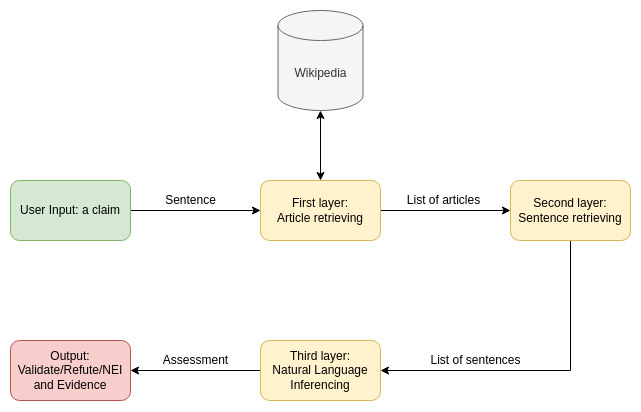
\includegraphics[scale=0.6]{img/use_case.png}
	\caption{General Model Processing Pipeline}
\end{figure}


\chapter{Identified challenges and solutions}
\section{Fact-Checking challenges}
In order for the model to work each layer/part of the system must answer to a specific task, the combination of results made by each layer constructs a robust model that is able with a degree of confidence to fact-check a claim as well as present evidence of the assessment. Although for each layer to work as intended we must find solutions to these challenges:\\

\begin{itemize}
	\item \textbf{Claims Spotting:} the model must be robust to linguistic changes, we must deal with different phrasing for the same or similar claims. For every "reasonable" input we must extract the target claim.
	\item \textbf{Articles Retrieving:} as Wikipedia holds millions of articles, the model must look for a limited number of relative articles to the input claim with an order of degree of correlation.
	\item \textbf{Time Recording:} relative articles in Wikipedia can be outdated, for example Britain belongs to the European Union is an outdated knowledge. The model must be sensitive to the timestamps of articles.
	\item \textbf{Sentences Retrieving:}  in each article retrieved from Wikipedia's database we must extract sentences relative to our input claim in order to apply a "kind of" comparison as well as present the winning sentences as evidence to the user.
	\item \textbf{Sentence Comparison:} here we must create a model or use a pre-existing natural language inferencing model in order to compare retrieved sentences from Wikipedia's articles and the input claim. 
	\item \textbf{Credibility Evaluation:} not all informations in Wikipedia are true.
\end{itemize}

These can be regarded as main challenges of our Fact-Checking project, but, evidently, other problems can be presented for example the verifiability of claims, not all claims can be verifiable, especially if it is an personal opinion or a personal belief, in this case the model must not give a True or False assessment but it should tell the user that there is not enough information (NEI) to make such an assessment.

\section{Related work and solutions}
\subsection{Styled based fake news detection}

\subsection{Propagation based fake news detection}

\subsection{Credibility based fake news detection}




\chapter{Conclusion}
Ces dernières années, de nombreuses techniques différentes de création d'empreintes digitales et d'indexation ont été proposées et sont maintenant utilisées dans des produits commerciaux. Dans ce projet, nous avons examiné de plus près l'une de ces techniques, qui a été développée à l'origine pour le système d'identification audio \textit{Shazam}. Nous avons discuté des idées principales qui sous-tendent ce système, mais il y a de nombreux paramètres qui doivent être ajustés afin de trouver un bon compromis entre les différentes exigences, notamment la robustesse, la spécificité, l'évolutivité et la compacité. Les aspects importants sont les suivants :\\

 \begin{itemize}
	\item les paramètres de la STFT (longueur de la fenêtre, taille du saut) qui déterminent les résolutions temporelle et spectrale,
	\item la stratégie de sélection et d'extraction des pics spectraux (avec ses paramètres de voisinage),
	\item la taille des zones cibles (utilisées pour définir les triplets), et
	\item des structures de données appropriées pour le hachage.
\end{itemize}

\vspace{0.5cm}
Bien que ce système est robuste à de nombreux types de distorsions du signal, l'approche de création d'empreinte discutée n'est pas conçue pour gérer les déformations temporelles. La correspondance des cartes de constellation ainsi que les différences d'horodatage (\textit{timestamp}) dans les paires de pics sont toutes deux sensibles aux différences de tempo relatif entre la requête et le document de base de données. Par conséquent, il est nécessaire d'utiliser d'autres techniques pour être invariant aux modifications de l'échelle de temps.\\

Les empreintes digitales utilisant les pics spectraux sont conçues pour être très sensibles à une version particulière d'un morceau de musique. Par exemple, face à une multitude d'interprétations différentes d'une chanson par le même artiste, le système d'empreintes digitales est susceptible de choisir la bonne, même si elles sont pratiquement indiscernables par l'oreille humaine. En général, les systèmes d'identification audio sont conçus pour cibler l'identification d'enregistrements qui sont déjà présents dans la base de données. Par conséquent, ces techniques ne sont généralement pas généralisables aux enregistrements en direct ou aux performances qui ne font pas partie de la base de données.


\chapter{Perspectives}
Comme décrit avant, il y a de nombreux paramètres qui doivent être ajustés afin de trouver un bon compromis entre les différentes exigences, notamment la robustesse, la spécificité, l'évolutivité et la compacité. Trouver des valeurs optimales à ces paramètres pourra augmenter largement les performances de notre application du point de vue de la robustesse aux distorsions, voire aussi du point de vue la mémoire utilisée et la vitesse de recherche d'une correspondance. Or, ce n'est pas une simple tâche, de plus les paramètres de notre application augmente, le processus de trouver des valeurs optimales à ces paramètres devient très compliqué.\\

Parmi les solutions que nous envisageons comme extension à notre application est l'utilisation d'un modèle de réseau neurones artificielles qui prendra en entrée les paramètres de notre application, et la sortie sera divisée sur les différentes exigences voulues tel que la robustesse, la mémoire, et le temps de recherche.\\

Ce réseau sera entraîné sur une large base d'apprentissage qui provienne de plusieurs tests déjà effectués d'une manière dynamique, par exemple nous allons exécuter la reconnaissance des morceaux sur une large collections de musiques tout en ajoutant du bruit et d'autres distorsions et aussi en variant le temps d'enregistrement du microphone, les résultats obtenus feront une très bonne base d'apprentissage pour notre réseau de neurones artificielles. Peut-être même on pourra ajuster les paramètres de notre application dynamiquement par rapport à chaque situation.\\


\begin{thebibliography}{100}
	 
	\bibitem{Wang} Avery L. Wang. An industrial-strength audio search algorithm. In \emph{Proceedings of the 4th Symposium Conference on Music Information Retrieval}, 2003.
	
	\bibitem{MG} Peter Grosche, Meinard Müller, and Joan Serrà: Audio Content-Based Music Retrieval. In \emph{Meinard Müller and Masataka Goto and Markus Schedl (ed.): Multimodal Music Processing, Schloss Dagstuhl—Leibniz-Zentrum für Informatik}, 2012.
	
	\bibitem{AI} Audio Identification : \href{https://www.audiolabs-erlangen.de/resources/MIR/FMP/C7/C7S1_AudioIdentification.html}{https://www.audiolabs-erlangen.de/resources/MIR/FMP/C7/C7S1\_AudioIdentification.html}.
	
	\bibitem{Kalker}  J. Haitsma, T. Kalker, and J. Oostveen, "Robust Audio
	Hashing for Content Identification". In \emph{n International Workshop on
		Content-Based Multimedia Indexing}, 2001.
	
	\bibitem{MG}  C.J. Burges, J. C. Patt, and S. Jana, “Distortion
	discriminant analysis for audio fingerprinting”. In \emph{IEEE
		Transaction on Speech and Audio Proc}, 2003.
	
	\bibitem{IEC} 6.050J/2.110J – Information, Entropy and Computation – Spring 2008  \href{https://mtlsites.mit.edu/Courses/6.050/2008/notes/mp3.html}{6.05https://mtlsites.mit.edu/Courses/6.050/2008/notes/mp3.html}.
	
	\bibitem{SCSS} Seeing circles, sines, and signals \href{https://jackschaedler.github.io/circles-sines-signals/sound.html}{https://jackschaedler.github.io/circles-sines-signals/sound.html}.
	
	\bibitem{PR}  Piotr Indyk, Rajeev Motwani. Approximate nearest neighbors: towards removing the curse of dimensionality.
	
	\bibitem{FA} Jerome Schalkwijk, A Fingerprint for Audio \href{https://medium.com/intrasonics/a-fingerprint-for-audio-3b337551a671}{https://medium.com/intrasonics/a-fingerprint-for-audio-3b337551a671}.
	
	\bibitem{PBAF} Jang et al. Pairwise Boosted Audio Fingerprint, 2009.
	
	\bibitem{STFT} Short-Time Fourier Transform. In \emph{Sensor Technologies for Civil Infrastructures}, 2014.
	
	\bibitem{FA} Nasser Kehtarnavaz. In \emph{Digital Signal Processing System Design (Second Edition)}, 2008.
	
\end{thebibliography}


\end{document}